% Rounding in Z[i]: any complex number (red) is within sqrt2/2 of the
% nearest Gaussian integer (blue lattice), shown by arrows.
% Source: book/tex/H113/ring-flavors.tex (§ Euclidean domains).
\documentclass[border=2mm]{standalone}
\usepackage{tikz}
\usetikzlibrary{arrows.meta}
\begin{document}
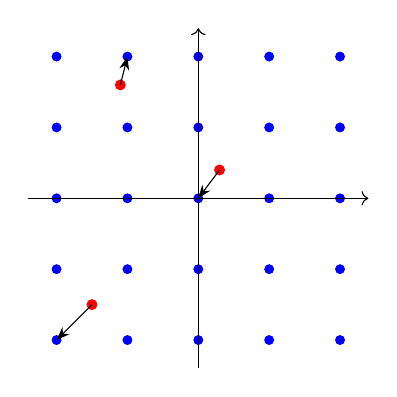
\begin{tikzpicture}[scale=0.9]
  \foreach \x in {-2,...,2}
    \foreach \y in {-2,...,2}
      \fill[blue] (\x,\y) circle (2pt);
  \foreach \px/\py/\rx/\ry in {0.3/0.4/0/0, -1.1/1.6/-1/2, -1.5/-1.5/-2/-2}{
    \fill[red] (\px,\py) circle (2.2pt);
    \draw[-{Stealth}] (\px,\py) -- (\rx,\ry);
  }
  \draw[->] (-2.4,0) -- (2.4,0);
  \draw[->] (0,-2.4) -- (0,2.4);
\end{tikzpicture}
\end{document}
